\section{Results}
\label{sec:results}

% Tables will be generated from benchmark data by scripts/generate-paper-tables.go
% and placed in paper/tables/

\subsection{Conformance}

All eight implementations (Go and Rust $\times$ \schubfach, \ryualg,
\dragonbox, and \burgerdybvig) pass the full conformance matrix: 776 total
cases (97~structural tests $\times$ 8~implementations, 0~failures).
Output SHA-256 digests are byte-identical across all implementations for
valid inputs.

\subsection{API Benchmarks}

API benchmarks isolate the algorithmic cost of the canonicalization
function, removing process startup and I/O overhead.  These measurements
most directly reflect the digit-generation performance difference.

Table~\ref{tab:api-summary} summarizes the key API results for the
within-language algorithm comparisons (canonicalize mode).
Figure~\ref{fig:api-speedup} visualizes the speedup across all shared
workloads for both language pairs.  Full results
for all pairs, modes, and workloads appear in
Appendix~\ref{sec:appendix-tables}.

% Auto-generated by scripts/generate-paper-tables.go
\begin{table}[htbp]
\caption{API benchmark summary: within-language algorithm comparisons (canonicalize mode, mean of $n{=}10$).}
\label{tab:api-summary}
\centering\small
\begin{tabular}{llrrr}
\toprule
Pair & Workload & \schubfach (ns/op) & \burgerdybvig (ns/op) & Speedup \\
\midrule
go:schubfach-vs-bd & array-2048 & 2541752 & 4077596 & 1.60$\times$ \\
go:schubfach-vs-bd & array-256 & 305467 & 473478 & 1.55$\times$ \\
go:schubfach-vs-bd & control-escapes & 1339 & 1258 & 1.06$\times$ \\
go:schubfach-vs-bd & deep & 36725 & 36749 & 1.00$\times$ \\
go:schubfach-vs-bd & deep-64 & 16230 & 16231 & 1.00$\times$ \\
go:schubfach-vs-bd & large & 11923743 & 20570122 & 1.73$\times$ \\
go:schubfach-vs-bd & long-string & 75831 & 75639 & 1.00$\times$ \\
go:schubfach-vs-bd & medium & 341106 & 582942 & 1.71$\times$ \\
go:schubfach-vs-bd & mixed-prod & 136352 & 180492 & 1.32$\times$ \\
go:schubfach-vs-bd & number-heavy & 13807 & 21412 & 1.55$\times$ \\
go:schubfach-vs-bd & numeric-boundary & 12693 & 18815 & 1.48$\times$ \\
go:schubfach-vs-bd & rfc-key-sorting & 3004 & 2973 & 1.01$\times$ \\
go:schubfach-vs-bd & small & 1251 & 1675 & 1.34$\times$ \\
go:schubfach-vs-bd & unicode & 1554 & 1551 & 1.00$\times$ \\
go:schubfach-vs-bd & verify-whitespace & 910 & 1569 & 1.72$\times$ \\
rs:schubfach-vs-bd & array-2048 & 1185768 & 2882258 & 2.43$\times$ \\
rs:schubfach-vs-bd & array-256 & 157030 & 321394 & 2.05$\times$ \\
rs:schubfach-vs-bd & control-escapes & 607 & 607 & 1.00$\times$ \\
rs:schubfach-vs-bd & deep-64 & 9380 & 9185 & 1.02$\times$ \\
rs:schubfach-vs-bd & long-string & 17259 & 17278 & 1.00$\times$ \\
rs:schubfach-vs-bd & numeric-boundary & 976 & 8975 & 9.19$\times$ \\
rs:schubfach-vs-bd & rfc-key-sorting & 1294 & 1250 & 1.04$\times$ \\
rs:schubfach-vs-bd & small & 583 & 1000 & 1.71$\times$ \\
rs:schubfach-vs-bd & unicode & 1676 & 1964 & 1.17$\times$ \\
rs:schubfach-vs-bd & verify-whitespace & 347 & 980 & 2.83$\times$ \\
\bottomrule
\multicolumn{5}{l}{\footnotesize Full results for all pairs, modes, and workloads in Appendix~\ref{sec:appendix-tables}.} \\
\end{tabular}
\end{table}


Table~\ref{tab:api-stats-summary} presents the within-language API
comparisons with BH-corrected $p$-values, confidence intervals, and
effect sizes.

% Auto-generated by scripts/generate-paper-tables.go
\begin{table*}[htbp]
\caption{Within-language API comparisons (canonicalize mode; BH-significant marked with $^*$).}
\label{tab:api-stats-summary}
\centering\small
\begin{tabular}{llllrrrrr}
\toprule
Pair & Workload & Winner & Speedup & CI$_{95}$ & $p_\text{adj}$ & $d$ & MDE (\%) \\
\midrule
go:schubfach-vs-bd & array-2048 & schubfach$^*$ & 1.57$\times$ & [1.558, 1.587] & 0.0003 & -48.58 & 1.8 \\
rs:schubfach-vs-bd & array-2048 & schubfach-rs$^*$ & 2.51$\times$ & [2.423, 2.548] & 0.0003 & -52.77 & 4.5 \\
go:schubfach-vs-bd & array-256 & schubfach$^*$ & 1.56$\times$ & [1.551, 1.567] & 0.0003 & -78.75 & 0.8 \\
rs:schubfach-vs-bd & array-256 & schubfach-rs$^*$ & 2.20$\times$ & [2.160, 2.258] & 0.0003 & -32.70 & 4.2 \\
go:schubfach-vs-bd & canonical-minimal & schubfach$^*$ & 1.54$\times$ & [1.529, 1.555] & 0.0003 & -47.74 & 1.7 \\
rs:schubfach-vs-bd & canonical-minimal & schubfach-rs$^*$ & 2.10$\times$ & [1.991, 2.205] & 0.0003 & -12.63 & 8.7 \\
go:schubfach-vs-bd & control-escapes & json-canon$^*$ & 1.06$\times$ & [1.035, 1.071] & 0.0005 & 2.81 & 2.9 \\
rs:schubfach-vs-bd & control-escapes & json-canon-rs & 1.02$\times$ & [0.961, 1.063] & 0.4784 & 0.37 & 9.7 \\
go:schubfach-vs-bd & deep-64 & json-canon & 1.00$\times$ & [0.999, 1.006] & 0.3660 & 0.44 & 0.5 \\
rs:schubfach-vs-bd & deep-64 & schubfach-rs & 1.00$\times$ & [0.979, 1.061] & 1.0000 & -0.01 & 0.8 \\
go:schubfach-vs-bd & deep & schubfach & 1.00$\times$ & [0.998, 1.006] & 0.3803 & -0.44 & 0.6 \\
rs:schubfach-vs-bd & deep & json-canon-rs$^*$ & 1.05$\times$ & [1.014, 1.094] & 0.0346 & 1.03 & 3.0 \\
go:schubfach-vs-bd & escaped-key-order & schubfach$^*$ & 1.60$\times$ & [1.593, 1.607] & 0.0003 & -80.96 & 0.6 \\
rs:schubfach-vs-bd & escaped-key-order & schubfach-rs$^*$ & 2.49$\times$ & [2.396, 2.546] & 0.0003 & -27.97 & 4.8 \\
go:schubfach-vs-bd & large & schubfach$^*$ & 1.72$\times$ & [1.707, 1.724] & 0.0003 & -92.98 & 0.8 \\
rs:schubfach-vs-bd & large & schubfach-rs$^*$ & 3.39$\times$ & [3.272, 3.453] & 0.0003 & -40.35 & 4.4 \\
go:schubfach-vs-bd & long-string & json-canon & 1.01$\times$ & [0.997, 1.025] & 0.2137 & 0.60 & 1.7 \\
rs:schubfach-vs-bd & long-string & json-canon-rs & 1.00$\times$ & [0.949, 1.030] & 0.8927 & 0.11 & 7.2 \\
go:schubfach-vs-bd & medium & schubfach$^*$ & 1.69$\times$ & [1.678, 1.703] & 0.0003 & -53.37 & 1.1 \\
rs:schubfach-vs-bd & medium & schubfach-rs$^*$ & 2.97$\times$ & [2.936, 2.996] & 0.0003 & -69.85 & 1.5 \\
go:schubfach-vs-bd & mixed-prod & schubfach$^*$ & 1.31$\times$ & [1.302, 1.317] & 0.0003 & -38.13 & 0.8 \\
rs:schubfach-vs-bd & mixed-prod & schubfach-rs$^*$ & 1.83$\times$ & [1.791, 1.856] & 0.0003 & -29.73 & 3.0 \\
go:schubfach-vs-bd & nested-mixed & schubfach$^*$ & 1.41$\times$ & [1.399, 1.413] & 0.0003 & -51.38 & 0.6 \\
rs:schubfach-vs-bd & nested-mixed & schubfach-rs$^*$ & 1.92$\times$ & [1.844, 1.959] & 0.0003 & -20.61 & 5.2 \\
go:schubfach-vs-bd & number-heavy & schubfach$^*$ & 1.56$\times$ & [1.547, 1.573] & 0.0005 & -43.14 & 1.3 \\
rs:schubfach-vs-bd & number-heavy & schubfach-rs$^*$ & 8.27$\times$ & [8.179, 8.374] & 0.0003 & -110.14 & 2.1 \\
go:schubfach-vs-bd & numeric-boundary & schubfach$^*$ & 1.49$\times$ & [1.482, 1.502] & 0.0003 & -48.06 & 1.1 \\
rs:schubfach-vs-bd & numeric-boundary & schubfach-rs$^*$ & 9.32$\times$ & [9.208, 9.424] & 0.0003 & -164.23 & 2.3 \\
go:schubfach-vs-bd & rfc-key-sorting & json-canon$^*$ & 1.02$\times$ & [1.011, 1.023] & 0.0003 & 2.41 & 0.9 \\
rs:schubfach-vs-bd & rfc-key-sorting & json-canon-rs & 1.01$\times$ & [0.967, 1.044] & 0.7629 & 0.15 & 6.3 \\
go:schubfach-vs-bd & small & schubfach$^*$ & 1.34$\times$ & [1.324, 1.345] & 0.0003 & -35.59 & 1.5 \\
rs:schubfach-vs-bd & small & schubfach-rs$^*$ & 1.75$\times$ & [1.712, 1.784] & 0.0003 & -22.01 & 3.1 \\
go:schubfach-vs-bd & surrogate-pair & json-canon$^*$ & 1.01$\times$ & [1.008, 1.019] & 0.0003 & 2.09 & 0.7 \\
rs:schubfach-vs-bd & surrogate-pair & json-canon-rs & 1.00$\times$ & [0.943, 1.075] & 0.9224 & 0.06 & 9.5 \\
go:schubfach-vs-bd & unicode & json-canon & 1.00$\times$ & [0.999, 1.009] & 0.2048 & 0.63 & 0.8 \\
rs:schubfach-vs-bd & unicode & schubfach-rs$^*$ & 1.03$\times$ & [1.005, 1.045] & 0.0277 & -1.13 & 3.6 \\
go:schubfach-vs-bd & verify-whitespace & schubfach$^*$ & 1.71$\times$ & [1.699, 1.723] & 0.0003 & -56.22 & 1.0 \\
rs:schubfach-vs-bd & verify-whitespace & schubfach-rs$^*$ & 2.90$\times$ & [2.831, 2.980] & 0.0003 & -30.28 & 4.2 \\
\bottomrule
\multicolumn{8}{l}{\footnotesize $^*$BH-significant at $q = 0.05$. $d$ = Cohen's $d$ ($\bar{x}_A - \bar{x}_B$)/$s_p$; negative = impl A faster.} \\
\multicolumn{8}{l}{\footnotesize MDE = minimum detectable effect at 80\% power. Full 317-comparison report in Appendix~\ref{sec:appendix-tables}.} \\
\end{tabular}
\end{table*}


\begin{figure*}[htbp]
\centering
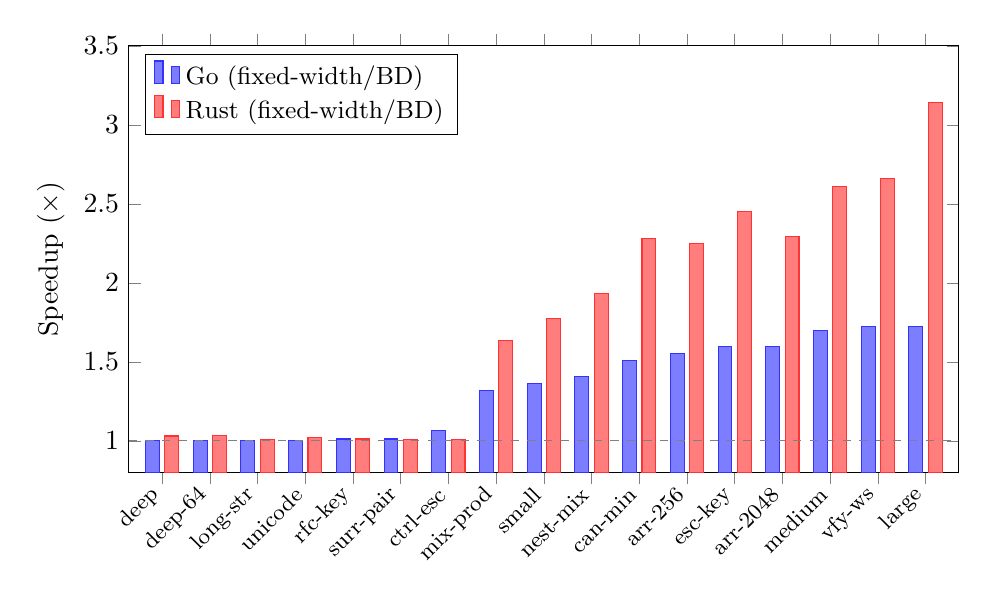
\begin{tikzpicture}
\begin{axis}[
    ybar,
    bar width=5pt,
    width=\textwidth,
    height=7cm,
    ylabel={Speedup ($\times$)},
    xtick={1,2,3,4,5,6,7,8,9,10,11,12,13,14,15,16,17},
    xticklabels={
        deep,
        deep-64,
        long-str,
        unicode,
        rfc-key,
        surr-pair,
        ctrl-esc,
        mix-prod,
        small,
        nest-mix,
        can-min,
        arr-256,
        esc-key,
        arr-2048,
        medium,
        vfy-ws,
        large},
    x tick label style={rotate=45, anchor=east, font=\footnotesize},
    ymin=0.8,
    ymax=3.5,
    xmin=0.3, xmax=17.7,
    ytick={1.0, 1.5, 2.0, 2.5, 3.0, 3.5},
    legend style={at={(0.02,0.98)}, anchor=north west, font=\small},
    legend cell align={left},
    every axis plot/.append style={fill opacity=0.85},
    clip=false,
]
% Go within-language (schubfach-vs-bd), sorted by Go speedup
% Pure-numeric outliers (numeric-boundary, number-heavy) shown separately in §8.5
\addplot[fill=blue!60, draw=blue!80] coordinates {
    (1, 1.000)
    (2, 1.000)
    (3, 1.001)
    (4, 1.003)
    (5, 1.012)
    (6, 1.012)
    (7, 1.065)
    (8, 1.320)
    (9, 1.364)
    (10, 1.408)
    (11, 1.509)
    (12, 1.552)
    (13, 1.595)
    (14, 1.599)
    (15, 1.698)
    (16, 1.721)
    (17, 1.724)
};
% Rust within-language (schubfach-vs-bd)
\addplot[fill=red!60, draw=red!80] coordinates {
    (1, 1.031)
    (2, 1.034)
    (3, 1.008)
    (4, 1.022)
    (5, 1.012)
    (6, 1.011)
    (7, 1.006)
    (8, 1.633)
    (9, 1.776)
    (10, 1.933)
    (11, 2.281)
    (12, 2.247)
    (13, 2.450)
    (14, 2.292)
    (15, 2.611)
    (16, 2.662)
    (17, 3.142)
};
\legend{Go (fixed-width/BD), Rust (fixed-width/BD)}
% Reference line at 1.0x
\draw[dashed, gray, thin] (axis cs:0.3,1.0) -- (axis cs:17.7,1.0);
\end{axis}
\end{tikzpicture}
\caption{API benchmark speedup of fixed-width over \burgerdybvig by
workload (canonicalize mode, \schubfach shown as representative;
\ryualg and \dragonbox produce equivalent ratios per
\S\ref{sec:results}).  Workloads sorted by Go speedup.  Values
above the dashed line indicate the fixed-width algorithm is faster.
Two pure-numeric workloads (\texttt{numeric-boundary} and
\texttt{number-heavy}) are presented separately in
\S\ref{sec:discussion} due to their degenerate number density
($\nu = 100\%$).  Number-dense workloads (right side) show the
largest advantage in both languages, consistent with a shared
algorithmic cause rather than language-specific runtime effects.}
\label{fig:api-speedup}
\end{figure*}


\subsection{Fixed-Width Algorithm Equivalence}

A central finding is that the three fixed-width algorithms (\schubfach,
\ryualg, \dragonbox) perform within 1--8\% of each other across both
languages and all workloads.  In Go API benchmarks, within-fixed-width
comparisons (go:schubfach-vs-ryu, go:schubfach-vs-dragonbox,
go:ryu-vs-dragonbox) show speedups of ${\leq}1.02\times$ with few
BH-significant differences.  In Rust, the same pattern holds, with
occasional small differences (${\leq}1.13\times$) reflecting
compilation artifacts rather than algorithmic cost.

This equivalence confirms that the dominant performance axis is
\emph{fixed-width vs.\ multiprecision}, not the choice among
fixed-width algorithms.

\subsection{CLI Benchmarks}

CLI benchmarks capture end-to-end pipeline cost including process
startup, argument parsing, file I/O, and output serialization.  Estimated
process startup overhead (approximately 1.3\,ms for Go, 0.5\,ms for Rust)
dominates for smaller workloads, attenuating the algorithmic signal
observed in API benchmarks.

Table~\ref{tab:cli-summary} summarizes the key CLI results.
Figure~\ref{fig:cli-significance} shows the end-to-end speedup with
BH-significance markers.  Full results appear in
Appendix~\ref{sec:appendix-tables}.

% Auto-generated by scripts/generate-paper-tables.go
\begin{table}[htbp]
\caption{CLI benchmark summary: within-language comparisons (canonicalize mode, $n{=}15$, 3 warmup discarded).}
\label{tab:cli-summary}
\centering\small
\begin{tabular}{llrrrr}
\toprule
Pair & Workload & Impl A (ms) & Impl B (ms) & Speedup & Winner \\
\midrule
go:schubfach-vs-bd & array-2048 & 5.466 & 7.063 & 1.29$\times$ & schubfach \\
go:schubfach-vs-bd & array-256 & 1.923 & 2.167 & 1.13$\times$ & schubfach \\
go:schubfach-vs-bd & canonical-minimal & 1.510 & 1.565 & 1.04$\times$ & schubfach \\
go:schubfach-vs-bd & control-escapes & 1.380 & 1.673 & 1.21$\times$ & schubfach \\
go:schubfach-vs-bd & deep-64 & 1.467 & 1.638 & 1.12$\times$ & schubfach \\
go:schubfach-vs-bd & escaped-key-order & 1.549 & 1.531 & 1.01$\times$ & json-canon \\
go:schubfach-vs-bd & long-string & 1.409 & 1.692 & 1.20$\times$ & schubfach \\
go:schubfach-vs-bd & nested-mixed & 1.511 & 1.497 & 1.01$\times$ & json-canon \\
go:schubfach-vs-bd & numeric-boundary & 1.537 & 1.706 & 1.11$\times$ & schubfach \\
go:schubfach-vs-bd & rfc-key-sorting & 1.561 & 1.608 & 1.03$\times$ & schubfach \\
go:schubfach-vs-bd & small & 1.450 & 1.449 & 1.00$\times$ & json-canon \\
go:schubfach-vs-bd & surrogate-pair & 1.510 & 1.524 & 1.01$\times$ & schubfach \\
go:schubfach-vs-bd & unicode & 1.597 & 1.470 & 1.09$\times$ & json-canon \\
go:schubfach-vs-bd & verify-whitespace & 1.455 & 1.614 & 1.11$\times$ & schubfach \\
rs:schubfach-vs-bd & array-2048 & 2.606 & 4.584 & 1.76$\times$ & schubfach-rs \\
rs:schubfach-vs-bd & array-256 & 0.828 & 1.152 & 1.39$\times$ & schubfach-rs \\
rs:schubfach-vs-bd & canonical-minimal & 0.546 & 0.582 & 1.07$\times$ & schubfach-rs \\
rs:schubfach-vs-bd & control-escapes & 0.531 & 0.594 & 1.12$\times$ & schubfach-rs \\
rs:schubfach-vs-bd & deep-64 & 0.564 & 0.647 & 1.15$\times$ & schubfach-rs \\
rs:schubfach-vs-bd & escaped-key-order & 0.573 & 0.712 & 1.24$\times$ & schubfach-rs \\
rs:schubfach-vs-bd & long-string & 0.605 & 0.636 & 1.05$\times$ & schubfach-rs \\
rs:schubfach-vs-bd & nested-mixed & 0.555 & 0.644 & 1.16$\times$ & schubfach-rs \\
rs:schubfach-vs-bd & numeric-boundary & 0.543 & 0.738 & 1.36$\times$ & schubfach-rs \\
rs:schubfach-vs-bd & rfc-key-sorting & 0.535 & 0.588 & 1.10$\times$ & schubfach-rs \\
rs:schubfach-vs-bd & small & 0.530 & 0.642 & 1.21$\times$ & schubfach-rs \\
rs:schubfach-vs-bd & surrogate-pair & 0.536 & 0.603 & 1.12$\times$ & schubfach-rs \\
rs:schubfach-vs-bd & unicode & 0.534 & 0.612 & 1.15$\times$ & schubfach-rs \\
rs:schubfach-vs-bd & verify-whitespace & 0.559 & 0.691 & 1.24$\times$ & schubfach-rs \\
\bottomrule
\multicolumn{6}{l}{\footnotesize Full results including verify mode and cross-language pairs in Appendix~\ref{sec:appendix-tables}.} \\
\end{tabular}
\end{table}


\begin{figure*}[htbp]
\centering
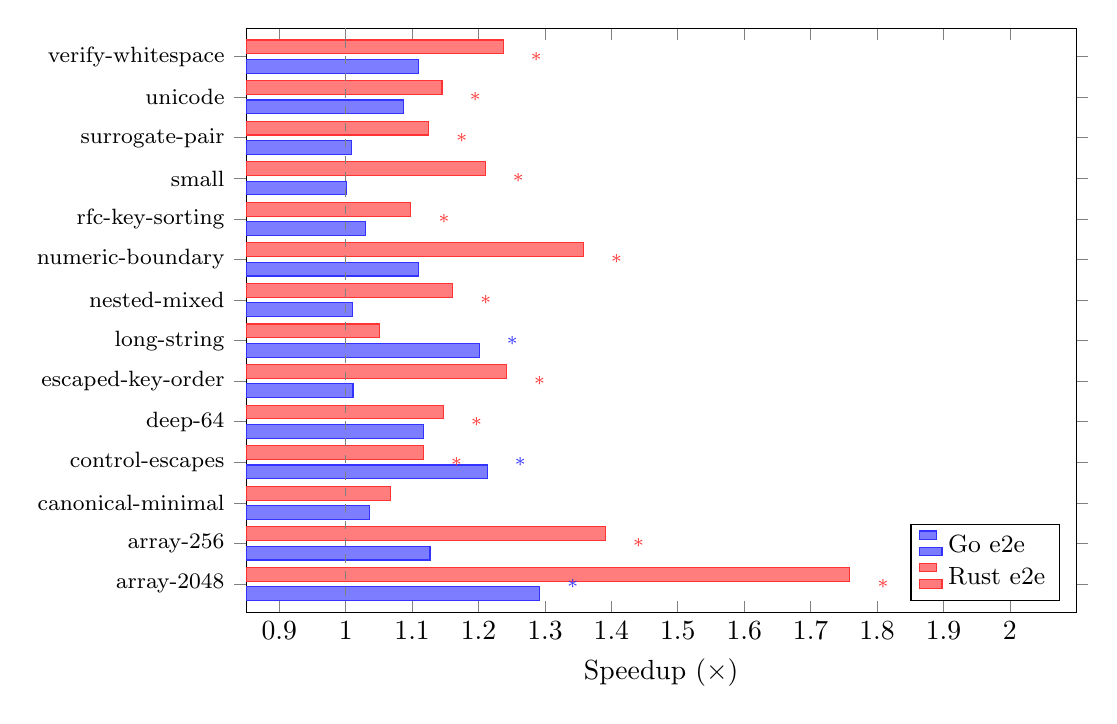
\begin{tikzpicture}
\begin{axis}[
    xbar,
    bar width=5pt,
    width=\textwidth,
    height=9cm,
    xlabel={Speedup ($\times$)},
    ytick={1,2,3,4,5,6,7,8,9,10,11,12,13,14},
    yticklabels={
        array-2048,
        array-256,
        canonical-minimal,
        control-escapes,
        deep-64,
        escaped-key-order,
        long-string,
        nested-mixed,
        numeric-boundary,
        rfc-key-sorting,
        small,
        surrogate-pair,
        unicode,
        verify-whitespace},
    y tick label style={font=\footnotesize},
    xmin=0.85,
    xmax=2.1,
    ymin=0.3, ymax=14.7,
    xtick={0.9, 1.0, 1.1, 1.2, 1.3, 1.4, 1.5, 1.6, 1.7, 1.8, 1.9, 2.0},
    legend style={at={(0.98,0.02)}, anchor=south east, font=\small},
    legend cell align={left},
    every axis plot/.append style={fill opacity=0.85},
    clip=false,
]
% Go CLI e2e canonicalize
\addplot[fill=blue!60, draw=blue!80] coordinates {
    (1.292, 1)
    (1.127, 2)
    (1.036, 3)
    (1.213, 4)
    (1.117, 5)
    (1.011, 6)
    (1.201, 7)
    (1.010, 8)
    (1.110, 9)
    (1.030, 10)
    (1.001, 11)
    (1.009, 12)
    (1.087, 13)
    (1.109, 14)
};
% Rust CLI e2e canonicalize
\addplot[fill=red!60, draw=red!80] coordinates {
    (1.759, 1)
    (1.391, 2)
    (1.067, 3)
    (1.117, 4)
    (1.147, 5)
    (1.242, 6)
    (1.051, 7)
    (1.161, 8)
    (1.358, 9)
    (1.098, 10)
    (1.210, 11)
    (1.125, 12)
    (1.145, 13)
    (1.237, 14)
};
\legend{Go e2e, Rust e2e}
% Reference line at 1.0x
\draw[dashed, gray, thin] (axis cs:1.0,0.3) -- (axis cs:1.0,14.7);
% BH-significant markers for Go (3 canonicalize: array-2048, control-escapes, long-string)
\node[font=\scriptsize, blue!80] at (axis cs:1.342, 1) {$*$};
\node[font=\scriptsize, blue!80] at (axis cs:1.263, 4) {$*$};
\node[font=\scriptsize, blue!80] at (axis cs:1.251, 7) {$*$};
% BH-significant markers for Rust (12 of 14 canonicalize)
\node[font=\scriptsize, red!80] at (axis cs:1.809, 1) {$*$};
\node[font=\scriptsize, red!80] at (axis cs:1.441, 2) {$*$};
\node[font=\scriptsize, red!80] at (axis cs:1.167, 4) {$*$};
\node[font=\scriptsize, red!80] at (axis cs:1.197, 5) {$*$};
\node[font=\scriptsize, red!80] at (axis cs:1.292, 6) {$*$};
\node[font=\scriptsize, red!80] at (axis cs:1.211, 8) {$*$};
\node[font=\scriptsize, red!80] at (axis cs:1.408, 9) {$*$};
\node[font=\scriptsize, red!80] at (axis cs:1.148, 10) {$*$};
\node[font=\scriptsize, red!80] at (axis cs:1.260, 11) {$*$};
\node[font=\scriptsize, red!80] at (axis cs:1.175, 12) {$*$};
\node[font=\scriptsize, red!80] at (axis cs:1.195, 13) {$*$};
\node[font=\scriptsize, red!80] at (axis cs:1.287, 14) {$*$};
\end{axis}
\end{tikzpicture}
\caption{CLI end-to-end speedup of \schubfach over \burgerdybvig by
workload (canonicalize mode, 15~repetitions each).  Asterisks ($*$) mark
BH-significant comparisons ($q < 0.05$).  The Rust within-language pair
achieves significance on 12 of 14~workloads; the Go pair on 3 of
14~workloads (canonicalize mode).  Process startup overhead
(${\approx}$1.3\,ms Go, ${\approx}$0.5\,ms Rust) attenuates the
algorithmic signal more strongly in Go.}
\label{fig:cli-significance}
\end{figure*}


\subsection{Statistical Comparisons}

Within-language CLI comparisons (canonicalize mode) with BH-corrected
$p$-values, confidence intervals, and effect sizes are reported in
Table~\ref{tab:stats-summary} (Appendix~\ref{sec:appendix-tables}).
The patterns mirror the API results: fixed-width algorithms outperform
\burgerdybvig on number-dense workloads, with smaller effect sizes due
to process startup dilution.  The full 1{,}644-comparison statistical
report appears in the supplementary materials.

\subsection{Cross-Language Validation}

All eight implementations pass the full conformance matrix (776 total
cases: 97~structural tests $\times$ 8~implementations, 0~failures) and
produce byte-identical output on all oracle vectors.  2{,}000
differential fuzz cases yield zero cross-implementation divergences.

The statistical report includes 16 comparison classes organized into
three groups:
\begin{itemize}
\item 6~within-Go algorithm pairs and 6~within-Rust algorithm pairs
      (testing algorithmic effects within each language),
\item 4~cross-language same-algorithm pairs (testing language/runtime
      effects while controlling for algorithm).
\end{itemize}

In CLI end-to-end measurement, Rust implementations are approximately
2--3$\times$ faster than their Go counterparts, primarily due to lower
process startup overhead (Rust native binary vs.\ Go runtime
initialization).  In API benchmarks, the within-Rust algorithmic ordering
replicates the within-Go ordering: all three fixed-width algorithms
outperform \burgerdybvig on number-dense workloads; this replication
of within-language ordering provides evidence that the fixed-width
advantage is not solely attributable to language-specific runtime
characteristics.

This decomposition separates algorithmic effects from language/runtime
effects and directly addresses language-specific performance threats.

\subsection{Differential Fuzzing}

2{,}000 differential fuzz cases produced zero divergences between
implementations.
